%\documentclass[slideColor,pdf, fyma2]{prosper}
\documentclass[svgnames]{beamer}
\usepackage{beamerthemesplit}
\usepackage{tikz}
\usepackage{xcolor}
\usepackage{verbatim}
\setbeamertemplate{navigation symbols}{} % Vypnuti navigation baru
\usepackage[utf8]{inputenc}
\usepackage[czech]{babel}
\newcommand{\myuv}[1]{\quotedblbase #1\textquotedblleft}
\setbeamertemplate{footline}{\hskip52em\textbf{\texttt{\insertframenumber/\inserttotalframenumber}}\vskip1em}
\setbeamertemplate{headline}{}
\setbeamertemplate{caption}{\insertcaption}
\setbeamertemplate{caption label separator}{}
%\setbeamertemplate{footline}[frame number]

\begin{document}
\title{Efektivní algoritmy pro práci s~konečnými automaty}
\author{Martin Hruška\\{\small Vedoucí: Ing. Ondřej Lengál}}

\frame{\titlepage} 

\frame{\frametitle{Motivace}
		\textcolor{Green}{Motivace}
		\begin{itemize}
			\item Konečné automaty
				\begin{itemize}
					\item Široké spektrum použití -- překladače, zpracování přirozeného jazyka, návrh číslicových systému, \textcolor{red}{formální verifikace}
					\item Algoritmy pro \textcolor{red}{nedeterministické} konečné automaty, především \textcolor{red}{test inkluze}
				\end{itemize}
		\end{itemize}

		\textcolor{Green}{Cíl}
		\begin{itemize}
			\item Vytvořit knihovnu pro práci s~konečnými automaty
		\end{itemize}
}

\frame{\frametitle{Definice NKA}
	\textcolor{red}{Nedeterministický konečný automat (NKA)} je pětice $(Q,\Sigma,\delta,S,F)$, kde
	\begin{itemize}
		\item $Q$ je konečná množina stavů
		\item $\Sigma$ je vstupní abeceda
		\item $\delta$ je přechodová funkce $Q\times\Sigma\rightarrow 2^Q$
		\item $S\subseteq Q$ je množina vstupních stavů
		\item $F \subseteq Q$ je množina koncových stavů
	\end{itemize}

  \begin{figure}[htp]
    \begin{center}
      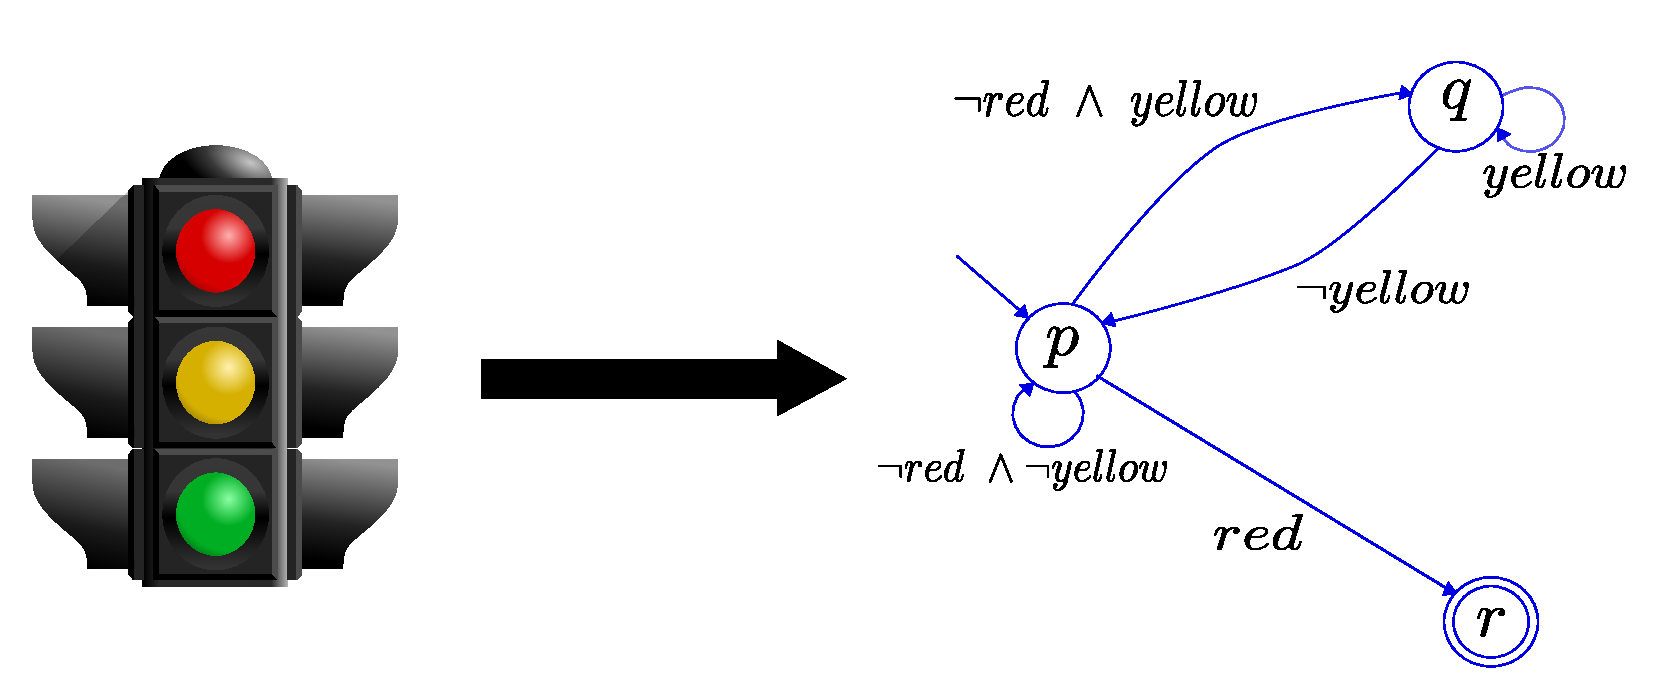
\includegraphics[scale=0.3]{tf_model.pdf}
    \end{center}
	\end{figure}
}


 \begin{comment}
		\begin{tikzpicture}[scale=0.09]
				\tikzstyle{every node}+=[inner sep=0pt]
				\draw [blue] (9.4,-29.6) circle (3);
				\draw (9.4,-29.6) node {$P$};
				\draw [blue] (29.9,-15.7) circle (3);
				\draw (29.9,-15.7) node {$Q$};
				\draw [blue] (29.9,-15.7) circle (2.4);
				\draw [blue] (33.8,-30.8) circle (3);
				\draw (33.8,-30.8) node {$R$};
				\draw [blue] (21.7,-50.3) circle (3);
				\draw (21.7,-50.3) node {$S$};
				\draw [blue] (21.7,-50.3) circle (2.4);
				\draw [blue] (51.1,-20.6) circle (3);
				\draw (51.1,-20.6) node {$T$};
				\draw [blue] (51.8,-41) circle (3);
				\draw (51.8,-41) node {$U$};
				\draw [blue] (51.8,-41) circle (2.4);
				\draw [blue] (3.2,-27.4) -- (6.57,-28.6);
				\fill [blue] (6.57,-28.6) -- (5.99,-27.86) -- (5.65,-28.8);
				\draw [blue] (11.88,-27.92) -- (27.42,-17.38);
				\fill [blue] (27.42,-17.38) -- (26.47,-17.42) -- (27.04,-18.25);
				\draw (20.6,-23.15) node [below] {$a$};
				\draw [blue] (10.93,-32.18) -- (20.17,-47.72);
				\fill [blue] (20.17,-47.72) -- (20.19,-46.78) -- (19.33,-47.29);
				\draw (14.9,-41.21) node [left] {$a$};
				\draw [blue] (12.4,-29.75) -- (30.8,-30.65);
				\fill [blue] (30.8,-30.65) -- (30.03,-30.11) -- (29.98,-31.11);
				\draw (21.33,-30.95) node [below] {$c$};
				\draw [blue] (32.82,-16.38) -- (48.18,-19.92);
				\fill [blue] (48.18,-19.92) -- (47.51,-19.26) -- (47.29,-20.23);
				\draw (39.8,-18.73) node [below] {$b$};
				\draw [blue] (36.38,-29.28) -- (48.52,-22.12);
				\fill [blue] (48.52,-22.12) -- (47.57,-22.1) -- (48.08,-22.96);
				\draw (43.5,-26.2) node [below] {$b$};
				\draw [blue] (36.41,-32.28) -- (49.19,-39.52);
				\fill [blue] (49.19,-39.52) -- (48.74,-38.69) -- (48.25,-39.56);
				\draw (41.85,-36.4) node [below] {$c$};
				\draw [blue] (48.93,-41.89) -- (24.57,-49.41);
				\fill [blue] (24.57,-49.41) -- (25.48,-49.66) -- (25.18,-48.7);
				\draw (35.85,-45.1) node [above] {$d$};
				\draw [blue] (32.22,-33.35) -- (23.28,-47.75);
				\fill [blue] (23.28,-47.75) -- (24.13,-47.33) -- (23.28,-46.81);
				\draw (27.12,-39.26) node [left] {$a$};
				\end{tikzpicture}
        \end{comment}



\frame{\frametitle{Algoritmy pro test jazykové inkluze}
		\textcolor{Green}{Klasický přístup}
		\begin{itemize}
			\item $L(A)\cap \overline{L(B)}=\emptyset$
			\item Nutná determinizace $\Rightarrow$ stavová exploze
		\end{itemize}

		\textcolor{Green}{Efektivní algoritmy}
		\begin{itemize}
			\item Umí pracovat s~nedeterministickými konečnými automaty
			\item	Nepotřebují vytvářet celý automat
			\begin{itemize}
				\item De Wulf, Doyen, Henzinger, Raskin. CAV'06.
				\item Abdulla, Chen, Holík, Mayr, Vojnar. TACAS'10.
				\item Bonchi, Pous. POPL'13.
			\end{itemize}
		\end{itemize}
		
		\begin{figure}
			\begin{tikzpicture}[scale=0.2]
				\draw (-3.0,-29.6) circle (6);
				\draw (0.0,-29.6) node {$B$};
				\filldraw [red] (-6.0,-29.6) circle (3);
				\draw (-6.0,-29.6) node {$A$};
			\end{tikzpicture}
		\caption{Inkluze}
		\end{figure}
}

\frame{\frametitle{Existující knihovny}
		\textcolor{Green}{dk.brics.automaton}
		\begin{itemize}
			\item balíček pro jazyk Java
			\item mutace \textcolor{red}{libfa} v~C a \textcolor{red}{fare} v~C\#
			\item pro test inkluze vyžaduje determinizaci
		\end{itemize}
		\textcolor{Green}{libgfsm, RWTH FSA Toolkit}
		\begin{itemize}
			\item starší knihovny v~C/C++
			\item opět problém s~nutností determinizace
		\end{itemize}
}			

\section{VATA}
\frame{\frametitle{VATA}
	\begin{itemize}
		\item Knihovna pro práci se \textcolor{red}{stromovými automaty}
		\item Zaměřena na oblast formální verifikace
		\item Podporuje explicitní a semi-symbolické kódování
		\item Cíl práce: rozšíření VATA pro \textcolor{red}{konečné automaty v~explicitním kódování}
	\end{itemize}
}

\section{Další postup}
\frame{\frametitle{Co bude ještě uděláno}
	\begin{itemize}
		\item Implementace algoritmů
		\item Testování a optimalizace
		\item Vyhodnocení výsledků práce
	\end{itemize}
}

\section{Závěr}
\frame{\frametitle{Závěr}
	\begin{center}
		\Large{\textbf{Děkuji za pozornost}}
	\end{center}
}
\begin{comment}

\frame{\frametitle{Obsah}
				\begin{center}
				\begin{tikzpicture}[scale=0.2]
				\tikzstyle{every node}+=[inner sep=0pt]
				\draw [red] (11.8,-11.4) circle (3);
				\draw [red] (11.8,-11.4) node {Úvod};
				\draw [black] (48.7,-18.1) circle (3);
				\draw (48.7,-18.1) node {KA};
				\draw [black] (10.1,-35.6) circle (3);
				\draw (10.1,-35.6) node {VATA};
				\draw [black] (48.7,-41.5) circle (3);
				\draw (48.7,-41.5) node {Závěr};
				\draw [black] (48.7,-41.5) circle (2.7);
				\draw [black] (6.5,-6.4) -- (9.62,-9.34);
				\fill [black] (9.62,-9.34) -- (9.38,-8.43) -- (8.69,-9.16);
				\draw [black] (14.75,-11.94) -- (45.75,-17.56);
				\fill [black] (45.75,-17.56) -- (45.05,-16.93) -- (44.87,-17.91);
				\draw [black] (45.97,-19.34) -- (12.83,-34.36);
				\fill [black] (12.83,-34.36) -- (13.77,-34.49) -- (13.35,-33.58);
				\draw [black] (13.07,-36.05) -- (45.73,-41.05);
				\fill [black] (45.73,-41.05) -- (45.02,-40.43) -- (44.87,-41.42);
				\end{tikzpicture}
				\end{center}
}

\section{Úvod} 
\frame{\frametitle{Úvod} 
	\begin{itemize}
		\item Vytvoření knihovny pro práci s~konečnými automaty
		\item Možnost testování inkluze konečných automatů -- využití ve formální verifikaci
		\item Realizace jako rozšíření knihovny VATA
	\end{itemize}
}

\frame{\frametitle{Zadání} 
	\begin{itemize}
		\item Studijnní část:
		\begin{itemize}
			\item Seznámit se s~teorií konečných automatů
			\item Seznámit se s~knihovnou VATA
	\end{itemize}
		\item Implementační část:
		\begin{itemize}
			\item Implementovat operace nad konečnými automaty
			\item Testování a vyhodnocení
		\end{itemize}
	\end{itemize}
}

\frame{\frametitle{Obsah}
				\begin{center}
				\begin{tikzpicture}[scale=0.2]
				\tikzstyle{every node}+=[inner sep=0pt]
				\draw [black] (11.8,-11.4) circle (3);
				\draw (11.8,-11.4) node {Úvod};
				\draw [red] (48.7,-18.1) circle (3);
				\draw [red] (48.7,-18.1) node {KA};
				\draw [black] (10.1,-35.6) circle (3);
				\draw (10.1,-35.6) node {VATA};
				\draw [black] (48.7,-41.5) circle (3);
				\draw (48.7,-41.5) node {Závěr};
				\draw [black] (48.7,-41.5) circle (2.7);
				\draw [black] (6.5,-6.4) -- (9.62,-9.34);
				\fill [black] (9.62,-9.34) -- (9.38,-8.43) -- (8.69,-9.16);
				\draw [black] (14.75,-11.94) -- (45.75,-17.56);
				\fill [black] (45.75,-17.56) -- (45.05,-16.93) -- (44.87,-17.91);
				\draw [black] (45.97,-19.34) -- (12.83,-34.36);
				\fill [black] (12.83,-34.36) -- (13.77,-34.49) -- (13.35,-33.58);
				\draw [black] (13.07,-36.05) -- (45.73,-41.05);
				\fill [black] (45.73,-41.05) -- (45.02,-40.43) -- (44.87,-41.42);
				\end{tikzpicture}
				\end{center}
}



\section{Operace pro konečné automaty}
\frame{\frametitle{Algoritmy pro konečné automaty}
	\begin{itemize}
		\item Operace -- sjednocení, průnik a především \textbf{test inkluze}
		\item Požadavek efektivity
		\begin{itemize}
			\item Použití efektivních algoritmů
			\item Implementační optimalizace
		\end{itemize}
		\begin{figure}
			\begin{tikzpicture}[scale=0.2]
				\draw (-3.0,-29.6) circle (6);
				\draw (0.0,-29.6) node {$B$};
				\filldraw [blue] (-6.0,-29.6) circle (3);
				\draw (-6.0,-29.6) node {$A$};

				%\filldraw [blue] (15.0,-29.6) circle (6);
				%\filldraw [blue] (21.0,-29.6) circle (6);
				
				%\filldraw [red] (36.0,-29.6) circle (6);
				%\filldraw [blue] (42.0,-29.6) circle (6);
			\end{tikzpicture}
		\caption{Inkluze}
		\end{figure}
	\end{itemize}
}

\frame{\frametitle{Efektivní algoritmy pro testování inkluze}
	\begin{itemize}
		\item Není třeba generovat všechny stavy
		\item Princip antichain a relace simulace
		\item Princip kongruence - především test ekvivalence, lze použít i pro inkluzi:
		\begin{itemize}
			\item $(X \cup Y = Y) \Rightarrow (X\subseteq Y)$
		\end{itemize}
	\end{itemize}
}
\begin{comment}
\frame{\frametitle{Obsah}
				\begin{center}
				\begin{tikzpicture}[scale=0.2]
				\tikzstyle{every node}+=[inner sep=0pt]
				\draw [black] (11.8,-11.4) circle (3);
				\draw (11.8,-11.4) node {Úvod};
				\draw [black] (48.7,-18.1) circle (3);
				\draw (48.7,-18.1) node {KA};
				\draw [red] (10.1,-35.6) circle (3);
				\draw [red] (10.1,-35.6) node {VATA};
				\draw [black] (48.7,-41.5) circle (3);
				\draw (48.7,-41.5) node {Závěr};
				\draw [black] (48.7,-41.5) circle (2.7);
				\draw [black] (6.5,-6.4) -- (9.62,-9.34);
				\fill [black] (9.62,-9.34) -- (9.38,-8.43) -- (8.69,-9.16);
				\draw [black] (14.75,-11.94) -- (45.75,-17.56);
				\fill [black] (45.75,-17.56) -- (45.05,-16.93) -- (44.87,-17.91);
				\draw [black] (45.97,-19.34) -- (12.83,-34.36);
				\fill [black] (12.83,-34.36) -- (13.77,-34.49) -- (13.35,-33.58);
				\draw [black] (13.07,-36.05) -- (45.73,-41.05);
				\fill [black] (45.73,-41.05) -- (45.02,-40.43) -- (44.87,-41.42);
				\end{tikzpicture}
				\end{center}
}

\section{VATA}
\frame{\frametitle{VATA}
	\begin{itemize}
		\item Knihovna pro práci se stromovými automaty
		\item Zaměřena na oblast formální verifikace
		\item Podporuje explicitní a semi-symbolickou kódování
		\item Cíl práce: rozšíření VATA pro konečné automaty v~explicitním kódování
	\end{itemize}

		\begin{figure}
			\begin{tikzpicture}[scale=0.1]
				\draw [blue] (41.8,-10.4) circle (3);
				\draw (41.8,-10.4) node {$f$};
				\draw [blue] (30,-21.3) circle (3);
				\draw (30,-21.3) node {$g$};
				\draw [blue] (41.8,-21.3) circle (3);
				\draw (41.8,-21.3) node {$a$};
				\draw [blue] (53.6,-22) circle (3);
				\draw (53.6,-22) node {$g$};
				\draw [blue] (24.5,-29.3) circle (3);
				\draw (24.5,-29.3) node {$a$};
				\draw [blue] (35.5,-30) circle (3);
				\draw (35.5,-30) node {$a$};
				\draw [blue] (48.3,-30.7) circle (3);
				\draw (48.3,-30.7) node {$a$};
				\draw [blue] (60.2,-30.7) circle (3);
				\draw (60.2,-30.7) node {$a$};
				\draw [blue] (32.2,-19.26) -- (39.6,-12.44);
				\draw [blue] (41.8,-18.3) -- (41.8,-13.4);
				\draw [blue] (51.46,-19.9) -- (43.94,-12.5);
				\draw [blue] (26.2,-26.83) -- (28.3,-23.77);
				\draw [blue] (33.9,-27.46) -- (31.6,-23.84);
				\draw [blue] (49.86,-28.14) -- (52.04,-24.56);
				\draw [blue] (58.39,-28.31) -- (55.41,-24.39);
			\end{tikzpicture}
		\caption{Stromový automat}
	\end{figure}			
}

\frame{\frametitle{Obsah}
				\begin{center}
				\begin{tikzpicture}[scale=0.2]
				\tikzstyle{every node}+=[inner sep=0pt]
				\draw [black] (11.8,-11.4) circle (3);
				\draw (11.8,-11.4) node {Úvod};
				\draw [black] (48.7,-18.1) circle (3);
				\draw (48.7,-18.1) node {KA};
				\draw [black] (10.1,-35.6) circle (3);
				\draw [black] (10.1,-35.6) node {VATA};
				\draw [red] (48.7,-41.5) circle (3);
				\draw [red] (48.7,-41.5) node {Závěr};
				\draw [red] (48.7,-41.5) circle (2.7);
				\draw [black] (6.5,-6.4) -- (9.62,-9.34);
				\fill [black] (9.62,-9.34) -- (9.38,-8.43) -- (8.69,-9.16);
				\draw [black] (14.75,-11.94) -- (45.75,-17.56);
				\fill [black] (45.75,-17.56) -- (45.05,-16.93) -- (44.87,-17.91);
				\draw [black] (45.97,-19.34) -- (12.83,-34.36);
				\fill [black] (12.83,-34.36) -- (13.77,-34.49) -- (13.35,-33.58);
				\draw [black] (13.07,-36.05) -- (45.73,-41.05);
				\fill [black] (45.73,-41.05) -- (45.02,-40.43) -- (44.87,-41.42);
				\end{tikzpicture}
				\end{center}
}

\section{Další postup}
\frame{\frametitle{Co bude ještě uděláno}
	\begin{itemize}
		\item Implementace algoritmů
		\item Testování a optimalizace
		\item Vyhodnocení výsledků práce
	\end{itemize}
}

\section{Závěr}
\frame{\frametitle{Závěr}
	\begin{center}
		\Large{\textbf{Děkuji za pozornost}}
	\end{center}
}
\end{comment}
\end{document}
